% !TeX encoding = UTF-8
%%%%%%%%%%%%%%%%%%%%%%%%%%%%%%%%%%%%%%%%%%%%%%%%%%%%%%%%%%%%%%%%%%%%%%%%%%%%%%%%
%2345678901234567890123456789012345678901234567890123456789012345678901234567890
%        1         2         3         4         5         6         7         8

\documentclass[a4paper, 10pt, conference]{ieeeconf}      % Use this line for a4
                                                          % paper

\IEEEoverridecommandlockouts                              % This command is only
                                                          % needed if you want to
                                                          % use the \thanks command
\overrideIEEEmargins
% See the \addtolength command later in the file to balance the column lengths
% on the last page of the document

% The following packages can be found on http:\\www.ctan.org
\usepackage{graphicx} % for pdf, bitmapped graphics files
%\usepackage{epsfig} % for postscript (.ps, .eps) graphics files
%\usepackage{mathptmx} % assumes new font selection scheme installed
%\usepackage{mathabx}
%\usepackage{times} % assumes new font selection scheme installed
\usepackage{amsmath} % assumes amsmath package installed
\usepackage{amssymb}  % assumes amsmath package installed
\usepackage[hidelinks]{hyperref}
\graphicspath{{img/}} % possible ot add more folders:
\graphicspath{{subdir1/}{subdir2/}{subdir3/}...{subdirn/}}
% or complete path (when figures are not in a subfolder of the main file)
%\graphicspath{{D:/LATEX/BEP/figures/}}




\title{\LARGE \bf
Measuring density of fluids in nanoliter volumes
}


\author{Michiel O'Herne (4387783), Joël van Beem (4487400),\\ Jan Vincent Hus (4299523) \\ % <-this % stops a space 
\supervisors{Dr. M.K. (Murali) Ghatkesar, Ir. T.G. (Tomas) Manzaneque}
%\thanks{Here you could add contact information, through which the interested reader may contact the author(s), such as %{\tt\footnotesize info@tudelft.nl}}
}
\date{December 22, 2019}


%%%%%%%%%%%%%%%%%%%%%%%%%%%%%%%%%%%%%%%%%%%%%%%%%%%%%%%%%%%%%%%%%%%%%%%%%%%%%%%%%%%
%%%%%%%%%%%%%%%%%%%%%%%%%%%%%%%%%%%%%%%%%%%%%%%%%%%%%%%%%%%%%%%%%%%%%%%%%%%%%%%%%%%
\begin{document}

% The three lines below print the title and page numbers, so please don't edit them
\maketitle
\thispagestyle{plain}
\pagestyle{plain}


%%%%%%%%%%%%%%%%%%%%%%%%%%%%%%%%%%%%%%%%%%%%%%%%%%%%%%%%%%%%%%%%%%%%%%%%%%%%%%%%
\begin{abstract}
    When measuring liquids with a resonating microbalance damping decreases the precision. To quantify this damping, the quality factor (Q factor)  is used, which is negatively correlated to the damping. A Quartz crystal was used to test and validate methods to improve this Q factor. Densities of different fluids were analyzed to validate practical use. Experimental data shows that the quality factor has increased by a factor 7x and density can be measured. 
\end{abstract}


%%%%%%%%%%%%%%%%%%%%%%%%%%%%%%%%%%%%%%%%%%%%%%%%%%%%%%%%%%%%%%%%%%%%%%%%%%%%%%%%
\section{Introduction}

    A Quartz-Crystal-Microbalance (a QCM) is a piezoelectric crystal that can be used as an acoustic wave microsensor to detect changes in density. QCMs are a highly effective tool at determining density at tiny liquid volumes. For example, observing the presence of E. coli bacteria in milk [X]. The presence of bacteria could be established in real time, instead of waiting for the outgrowth of bacteria in a laboratory.\\

    The density frequency relationship for small solid particles was first introduced by Sauerbrey (1959) [3] and later extended to describe liquid loading by Gordon and Kanazawa et al. (1985) [5]. More recently Kirkendall. et al (2010) [10] have explored how to increase precision by introducing an isolation layer on the QCM and almost eliminated damping effects of liquid loads. \\

    The achieved quality factor, defined as $Q=f0/ \Delta f_{3db}$ with $f0$ being the resonance frequency and $\Delta f_{3db}$ the bandwidth respectively, was recorded as 1600. Standard commercially available devices such as the OpenQCM record a quality factor of 3000. \\

    This observation has lead to an exploration whether further decrease of damping effects is possible. The central thesis of this paper is defined as: “Damping effects of liquids can be decreased by restricting the freedom of movement of the liquid, along with removing contact between crystal and liquid”.\\
%%%%%%%%%%%%%%%%%%%%%%%%%%%%%%%%%%%%%%%%%%%%%%%%%%%%%%%%%%%%%%%%%%%%%%%%%%%%%%%%
\section{Method}
\begin{itemize}
  \item    Why is the chosen methodology appropriate? Choice of experiments and design parameters is clearly described. 
  \item    Another person could replicate your study based on reading your method section > Procedure. 
  \item    A reader could evaluate your study well enough to tell whether your conclusions are valid.
  \item    Sometimes you describe at the beginning of the method section the task and experiment you did. 
  \item    Give a 2 sentence summary of your results.
\end{itemize}

\subsection{Choice of experiments}
    The QCM was loaded with fluid containers to test the hypothesis. Fluid containers were chosen because this allows to both restrict fluid movement and limit contact between crystal and fluid. Two main concepts have been tested to compare the damping effects of different shapes and volumes: (i) ceramic micro capillaries, (ii) plastic tubes. In addition, several attachment methods to attach the fluid container to the QCM were tested: (i) Clamping between blocks, (ii) Clamping with O-rings, (iv) Clamping with foam. (v) Glue.\\

    Tubular concepts were chosen over compartment based concepts as tubular concepts allow fluid to flow through the device. Which is often required for practical research or industrial use, as this allows the device to stay calibrated throughout multiple experiments. \\
    
    
%%%%%%%%%%%%%
\subsection{experimental setup procedure}
    The experiments were conducted in the following order:
\begin{itemize}
    \item    Unloaded 
    \item    Loaded with empty container 
    \item    Loaded with isopropanol filled container 
    \item    Loaded with deminiralized water filled container 
\end{itemize}
    These tests were done with a 90 and 180 degree rotation in respect to mount (see figure). In total there were 8 tests per setup.\\
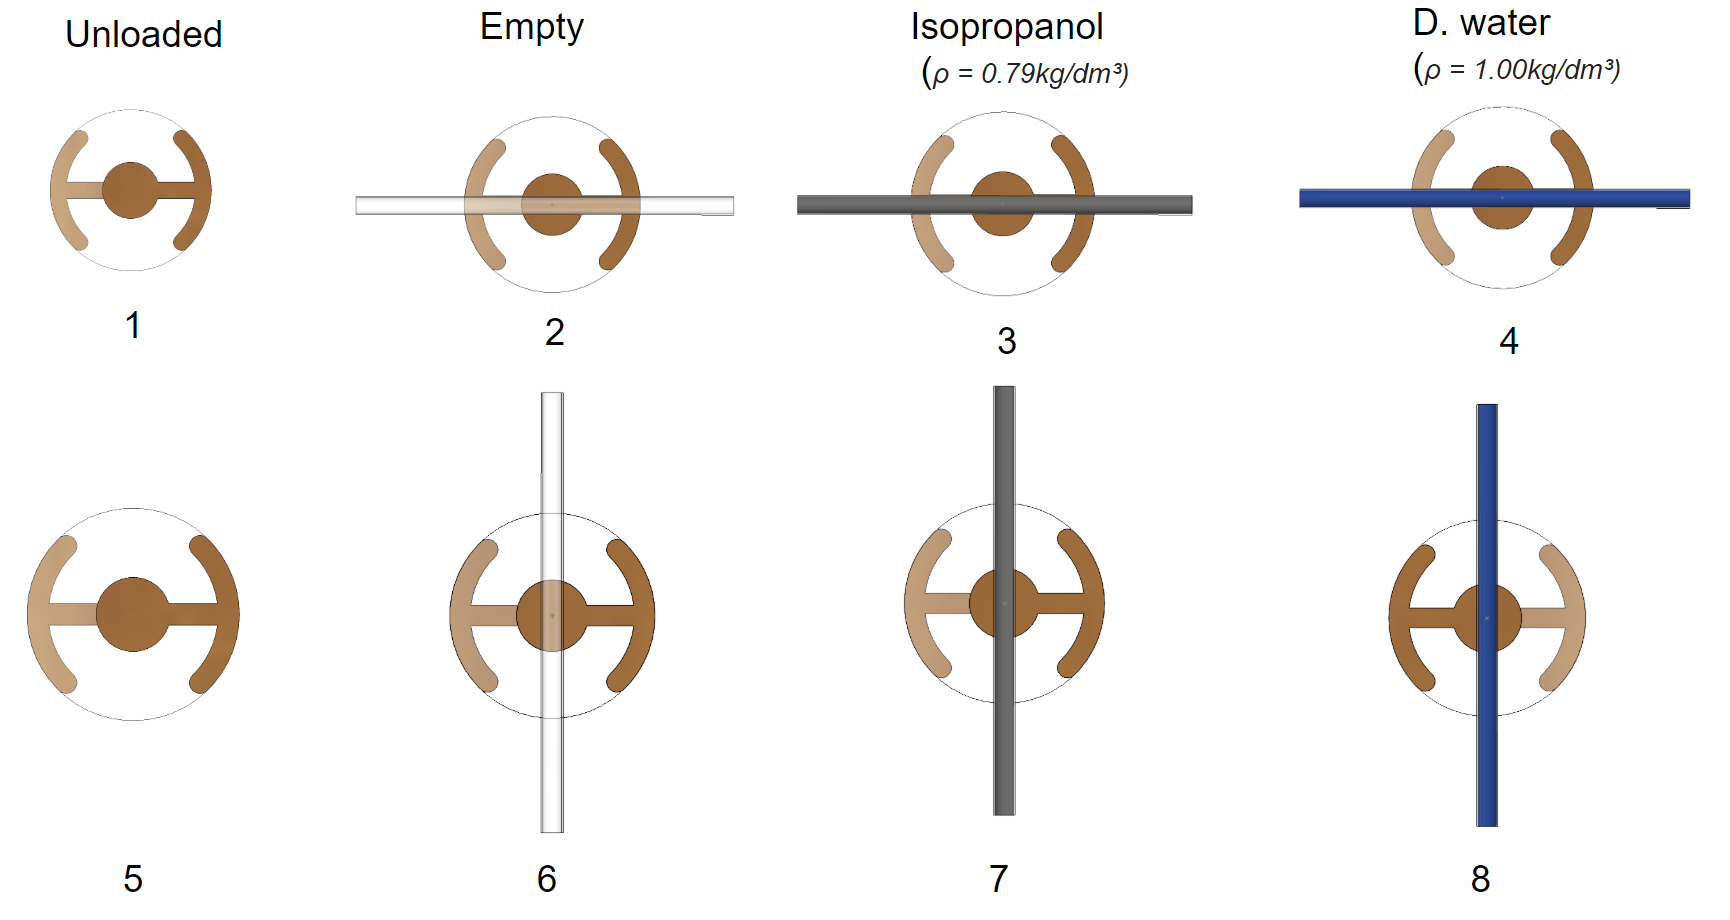
\includegraphics[scale=0.2]{setup.png}


%%%%%%%%%%%%%
\subsection{Fabrication}
    To conduct the experiments a device was fabricated that was connected to the network analyzer. 
    The frame was 3D printed and kept the quartz crystal, fluid container and electrical wiring together.
    A schematic of the final iteration with key components are shown in the figure X below: (a) crystal mount, (b) electrical wiring, (c) 5 MHz quartz crystal, (d) 25$\mu$L ceramic capillary.\\
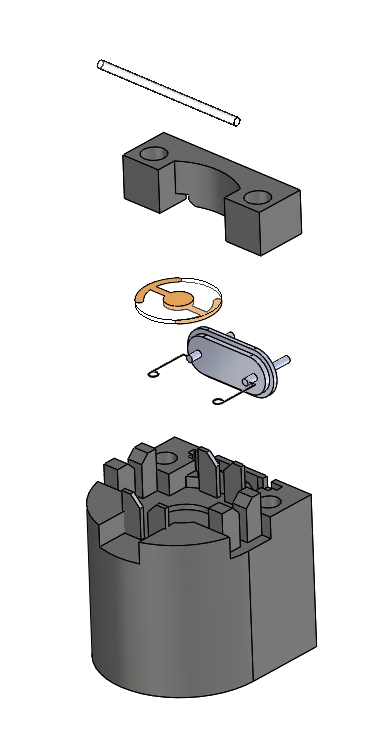
\includegraphics[scale=0.5]{capillary.PNG} \\

    The device has been designed with a modularized approach in mind so that separate components could be switched during the experiments. For instance, two separate mounts were used respectively for the capillary and polymer tube as was required due to their different shape and size: 
\begin{itemize}
    \item Ceramic capillary (25$\mu$L)
    \item Polymer tube (id = 4mm, od = 5mm)
\end{itemize}



%%%%%%%%%%%%%
\subsection{Measurement}
    Measurements were conducted by doing a frequency sweep on the loaded QCM using a Network Analyzer that measured the reflection loss factor (s11) from which the conductance from which the impedance can be determined as
    $Z = Z0* \frac{(1+S11)}{(1-S11)}$ and for the conductance
    $G= 1/Z$. 
    The conductance was plotted against the frequency and the quality factor determined as the resonance frequency divided by the bandwidth or twice the frequency difference at 3dB cutoff height of the conductance. 
    Over 250 data samples were collected and processed using python. \\
    
%%%%%%%%%%%%%%%%%%%%%%%%%%%%%%%%%%%%%%%%%%%%%%%%%%%%%%%%%%%%%%%%%%%%%%%%%%%%%%%%
\section{Results}
\subsection{Fluid containers compared to direct loading}
    Reference benchmarks were established by taking measurements with an unloaded QCM (air) and an empty capillary loaded on the fabricated QCM device. 
    For the unloaded situation a median Q-factor of ≈ 43.000 was noted. For the empty capillary the Q-factor median decreased  26.000. \\

    To evaluate the main hypothesis drops of demineralized water (around 20-30$\mu$L) were placed directly on the fabricated device. 
    This was compared to loading the QCM with ceramic capillaries (25L) and polymer tubes (XL) containing demineralized water.
    Figure X shows the Q-factor median and result range obtained for each configuration. \\

    A significantly higher Q-factor can be observed.
    When the liquid was placed directly on the surface of QCM a Q-factor of around 1000-4000 was observed.
    When the QCM is loaded with the liquid placed inside a fluid container, Q-factor ranges of 16.000  to 39.000 can be observed with the median hovering slightly above 25.000.
    These results show alignment with the hypothesis and indicate that the Q-factor is improved by over 7 times.\\


%%%%%%%%%%%%%
\subsection{Density detection}
    Experiments with demineralized water and Isopropanol were conducted to analyze the relationship between $\Delta$ mass and frequency shift when the liquid is placed inside a container.
    Figure 3 presents the data for demineralized water ($\rho$ 1.00 kg/dm3) and isopropanol ($\rho$ 0.79 kg/dm3).
    The median frequency shift for demineralized water was 24 Hz and for isopropanol 19 Hz.
    This corresponds to the difference in density between both liquids. \\
    
    
%%%%%%%%%%%%%
\subsection{Variance between results}
    The data shows significant amounts of deviation from the median between the results.
    It was observed that this was only the case when the load was moved or replaced between experiments.
    This in contrast to the consistent results when repeating experiments and without moving the load.
    When taking a large enough sample size the median does converge to expected values as can be seen in section 4.2 about density experiments. \\

    The data shows significant amounts of deviation from the median between the results.
    It was observed that this was only the case when the load was moved or replaced between experiments.
    This in contrast to the consistent results when repeating experiments and without moving the load.
    When taking a large enough sample size the median does converge to expected values as can be seen in section 4.2 about density experiments. \\
    
    The mass sensitivity is different at local positions and can be observed when examining a displacement model in COMSOL as shown in the figure X.
    An assumption can be made that if the load is placed with a non-uniform mass distribution in the longitudinal oscillation direction, the position is of much higher influence on the mass sensitivity than when placed across the oscillation direction. \\


%%%%%%%%%%%%%
\subsection{Oscillation direction}
    Experiments with demineralized water and Isopropanol were conducted to analyze the relationship between $\Delta$ mass and frequency shift when the liquid is placed inside a container.
    Figure 3 presents the data for demineralized water ($\rho$ 1.00 kg/dm3) and isopropanol ($\rho$ 0.79 kg/dm3).
    The median frequency shift for demineralized water was 24 Hz and for isopropanol 19 Hz.
    This corresponds to the difference in density between both liquids. \\
    
    
%%%%%%%%%%%%%
\subsection{Theoretical models versus experimental data}
    Water-drop experiments were conducted with water droplets of a weight of around 6$\mu$ which in theory should yield a frequency shift of 693 Hz (6$\mu$g*56.6Hz*$\mu$-1*cm2/0.49cm2).
    This is a similar outcome to a QCM fully immersed in water which yields a frequency shift of 714Hz, as per the Gordon Kanawaza equation. \\

    Thus the Sauerbrey and Gordon Kanawaza equations yield results in comparable orders of magnitude.
    It is important to note that both equations assume a uniformly distributed mass.
    However during this research situations with non-uniform mass distributions were analyzed, capillaries and tubular constructs in particular.
    As might be expected, the results from the theoretical model differ significantly from the experiments as described in section ‘results from experiments’.
    For Setup 3, the frequency shift for 25$\mu$ water injected in a capillary was 37.5Hz.  \\

    These differences can in part be explained that the mass sensitivity of QCMs differ greatly depending on the mass placed from the distance of the center [6].
    To this extend alternative models have been explored that have made attempts at overcoming these issues such as Huang et al. (2017) [7] where the mass sensitivity factor $C_f$ is described as a function of the radius of the electrodes and distance of the particle with respect to the center: \\

    However, for a 5 MHz crystal mass sensitivity factor can differ only by 1.2x to 2.6x which is far smaller than the 20x (37.5/714) ratio that we encountered. As such only a limited model for the specific conditions in this research has been made based on data correlations. \\



%%%%%%%%%%%%%%%%%%%%%%%%%%%%%%%%%%%%%%%%%%%%%%%%%%%%%%%%%%%%%%%%%%%%%%%%%%%%%%%%
\section{Discussion and Recommendation}
    With technological advancements happening more frequently on a nano scale, the need for sensors with such resolution will continue to rise.
    Therefore this area of research shows a lot of promise. Below a couple recommendations are described for future improvements. \\

    The area that has the most potential for improvement is consistency of the experiment setup.
    If the current standard deviation of X is brought down to an acceptable level of X it could be applied in industrial applications. \\

    Future research could be to pursue a setup with uniform mass distribution, as this would allow existing theoretical models to be used.
    Results could then be more effectively be verified with precise calculations.
    An idea would be to use flat layers that uniformly cover the area of the QCM membranes and foiles to separate the liquid from the QCM and contain the fluid. \\

    With a uniform mass distribution, the expected frequency shift would be roughly 20x times larger which would influence the precision as the measurable frequency shift is 0.1 Hz. \\

    Figure 11 shows the median Frequency shift and 50$\%$ ranges belonging to the experiments with different fluid containers and water loads. This figure illustrates the high amount of overlapping that exists over the ranges. In this case Isopropanol is ≈ 20$\%$ lower density than water. \\

    One of the key findings of the research was the extreme sensitivity to positioning of the load on the QCM. To this extend a completely consistent positioning of the capillary should improve reproducibility. The position angle relative to the oscillation direction of the crystal has shown promising results as well. \\


%%%%%%%%%%%%%%%%%%%%%%%%%%%%%%%%%%%%%%%%%%%%%%%%%%%%%%%%%%%%%%%%%%%%%%%%%%%%%%%%
\section{Conclusions}
    Damping effects of liquid loaded QCM measurements have been decreased by the use of ceramic capillaries.
    Inline with the hypothesis, the measured Quality-factor has been consistently higher when placing the fluid inside of a fluid container.
    The Quality factor has improved by a range of 7x to 9x. \\

    During the experiments capillaries and other fluid containers were placed on the QCM and loaded with fluid.
    To make sure this was done as accurately as possible, a 3D printed construct was designed to hold the quartz crystal, fluid container and electrical wiring together.
    Clamping mechanisms were found to be most effective. It was not possible to bring the QCM in resonance after gluing a capillary on the surface.
    The construct is modularized allowing parts to be exchanged which is required when testing different clamping methods or tubing. \\

    To make sure this was done as accurately as possible, fluids with varying densities, different setups, and positioning angles with regards to the crystal oscillation direction were tested throughout the research.
    The frequency shift was found to be extremely sensitive to the positioning of the load and the results between experiments where the load was moved or changed were inconsistent.
    The oscillation direction was found to be of influence and a load position angle of 90° was found to yield more consistent results compared to 180°. \\

    Measurements were conducted by doing a frequency sweep on the loaded QCM using a Network Analyzer that measured the reflection loss factor (s11) from which the conductance, resonance frequency and quality factor were calculated using python.
    The results with regards to the frequency shift were inconsistent and it was not possible to correlate mass-frequency shifts for individual experiments.
    When taking the average of a large experiment sample, a more accurate linear relationship should be observable. \\



%%%%%%%%%%%%%%%%%%%%%%%%%%%%%%%%%%%%%%%%%%%%%%%%%%%%%%%%%%%%%%%%%%%%%%%%%%%%%%%%
\section*{References}

[1]  Mecea, V.M. (2005), From Quartz Crystal Microbalance to Fundamental Principles of Mass Measurements. \\

[2] Mechale,  G. (2008), Density−Viscosity Product of Small-Volume Ionic Liquid Samples Using Quartz Crystal Impedance Analysis. \\

[3] Sauerbrey, G. H. (1959), Use of quartz vibration for weighing thin films on a microbalance. \\

[4] K.K Kanazawa, J.G Gordon (1985), The oscillation frequency of a quartz resonator in contact with liquid. \\

[5] Stanford Research Systems (2003), QCM100- Quartz Crystal Microbalance Theory and Calibration. \\

[6] John R. Vig, (1998), Comments About the Effects of Nonuniform Mass Loading on a Quartz Crystal Microbalance. IEEE transactions on ultrasonics, ferroelectrics, and frequency control. \\

[7] Huang, X., Bai, Q. et al. (2017) A Practical Model of Quartz Crystal Microbalance in Actual Applications. \\

[8] Rodahl, M. et al. (1997) QCM Operation in Liquids: An Explanation of Measured Variations in Frequency and Q Factor with Liquid Conductivity \\

[9]  Lee, W. et al. (2014) 3D-Printed Microfluidic Device for the Detection of Pathogenic Bacteria Using Size-based Separation in Helical Channel with Trapezoid Cross-Section.
https://www.ncbi.nlm.nih.gov/pmc/articles/PMC4289896/pdf/srep07717.pdf \\

[10] Kirkendall, C.R. et al. (‎2009), Liquid Damping Isolation on Quartz Crystal Microbalance for Effective Preservation of High Quality Factor and Sensitivity in Liquid \\

[11] Rodríguez-Pardo, L. et al.  (2005),Sensitivity, Noise, and Resolution in QCM Sensors in Liquid Media \\



%%%%%%%%%%%%%%%%%%%%%%%%%%%%%%%%%%%%%%%%%%%%%%%%%%%%%%%%%%%%%%%%%%%%%%%%%%%%%%%%
%\subsection{Layout guidelines}
%In this subsection the guidelines for the layout are given.
%\begin{itemize}
%	\item The BEP paper has to be written in English. 
%	\item Minimum number of pages = 6, maximum number is 10.
%	\item The formatting is taken care of by the \texttt{ieeeconf}-package, please do not change this.
%\end{itemize}


%\subsection{Including figures and tables}

%Put captions under figures and tables, which can be done by using the \texttt{caption}-command. Never include a figure or table in the paper without any reference to it in the text. An example of a figure is shown in Fig.~\ref{fig:example} and an example of a table is Table~\ref{tab:example} (by the way, the `$\sim$' symbol is used to add a space between two words, but to prevent them being on different lines). In general \LaTeX\ will put the figures and tables on the \textit{best} place it can find, near the text where it is inserted in the \texttt{tex} code. As a rule of thumb, try to make sure that a figure or table ends up on the same (or if not possible, the next) page as where you refer to it for the first time. 

%\subsubsection{Figures}
%A figure is included using some specific commands, see Fig.~\ref{fig:example}. Many kinds of image file formats are supported, such as:
%\begin{enumerate}
%	\item Portable network graphics (PNG)
%	\item Joint Photographic Experts Group (JP(E)G)
%	\item Portable Document Format (PDF)
%	\item Etcetera (BMP, EPS, PS, ...).
%\end{enumerate}

%\begin{figure}
%	\centering
%	\includegraphics[width=\columnwidth]{img/people}
%	\caption{Natural people will be outnumbered soon. When writing papers, it is good practice to create figures that are useful when printed in one column. Try to make sure that text and / or numbers within your figure are readable when printed in this size.}
%	\label{fig:example}
%\end{figure}
%
%\begin{table}[h]
%	\caption{An Example of a Table}
%	\label{tab:example}
%	\centering
%	\begin{tabular}{|c||lr|r|}
%		\hline
%		One & Two & Three & Four\\ \hline
%		Five & Six & \multicolumn{2}{|c|}{Seven and Eight}\\ 
%	\end{tabular}
%\end{table}

%\subsubsection{Tables} 
%Tables are included in a document using some specific commands as well, see Table~\ref{tab:example}. For constructing tables with complex shapes, try to search the web for instance for `\texttt{latex table}'. By the way, the `table' and `figure' environments decide for themselves what the best position is, in most cases this will be on the top of some column. One can force such `floating' environments to be placed where they are entered in the text by adding `[h]' directly after the environment declaration:

%%%%%%%%%%%%%%%%%%%%%%%%%%%%%%%%%%%%%%%%%%%%%%%%%%%%%%%%%%%%%%%%%%%%%%%%%%%%%%%%
 






%%%%%%%%%%%%%%%%%%%%%%%%%%%%%%%%%%%%%%%%%%%%%%%%%%%%%%%%%%%%%%%%%%%%%%%%%%%%%%%%
%\LaTeX\ is especially suited for editing and printing complex equations, such as the one in (\ref{eq:example1})\footnote{This ``(1)'' is the preferred way of refering to equations / mathematical expressions that are numbered.}. 

%\begin{equation} \label{eq:example1}
%	L' = {L}{\sqrt{1-\frac{v^2}{c^2}}}
%\end{equation}

%Equations / math can be entered in various ways, including more than one line at a time, using `align' (\ref{eq:align0}, \ref{eq:align1}). This can be done with or without a \texttt{subequations} environment:

%\begin{subequations}
%	\begin{align}
%%		\dot{x_1} &= 2 x_1 + \mu x_2\label{eq:align0}\\
%		\dot{x_2} &= x_1 + \alpha \sin(x_2)\label{eq:align1}
%	\end{align}	
%\end{subequations}

%Or, as in (\ref{eq:align2}) and (\ref{eq:align3}):

%\begin{align}
%	f(x)  &= a x^2+b x +c   &   g(x)  &= d x^3 \label{eq:align2}\\
%	f'(x) &= 2 a x +b       &   g'(x) &= 3 d x^2\label{eq:align3}
%\end{align}

%In general, see \url{https://en.wikibooks.org/wiki/LaTeX} for many more examples on how to include math in your document. Two last tips: when you use some functions that are described by letters (such as the sinus, or logarithm), always start them with a slash. Otherwise the letters will look like variables: $y = \sin(x)$ or $y = sin(x)$ (by the way, the dollar signs let you use math outside of the official \textit{equations}-environments). The other tip is to always (always!) declare the variables that you use somewhere in your text, either in a small (sub) section following your introduction, or where ever you first use them. 

%%%%%%%%%%%%%%%%%%%%%%%%%%%%%%%%%%%%%%%%%%%%%%%%%%%%%%%%%%%%%%%%%%%%%%%%%%%%%%%%

%There are many ways to include references in your \LaTeX\ document, such as \cite{AbedonHymanThomas2003}. In this template we use \textit{BibTex}, which is one of the more automated ways of taking care or your referencing. Notice that when you change the \texttt{paper.bib}-file, you need to run \texttt{bibtex paper} in order to include the changes that you have made in the document. When you use a proper editor for writing your \LaTeX\ -document, this will probably be taken care of automatically.

%References are listed at the end of the paper. Never put a reference in the list of references without referencing to it in the text, and try to use references that make sense to include in your document \cite{einstein1935can}.

%%%%%%%%%%%%%%%%%%%%%%%%%%%%%%%%%%%%%%%%%%%%%%%%%%%%%%%%%%%%%%%%%%%%%%%%%%%%%%%%

%This section gives guidelines for the structure of the BEP paper. A scientific paper/report usually contains the following elements:

%\begin{itemize}
%	\item Give a motivation for the present study and some background information when necessary: what is the relevance of your project from a societal, environmental, political and/or economic point of view?
%	\item What is the relevance of the project from a scientific point of view? Briefly review the literature: what has already been done and what are open questions?
%	\item Formulate the scientific objectives of the present study. What are the questions that you want to answer and/or what are the hypotheses you want to check? 
%	\item How are you going to reach your goal(s) or going to answer your research question(s)? Give a concise and brief description of the approach taken / the methodology used. You will discuss this further in a separate section later on in the paper.
%	\item Briefly describe the setup / sections of the paper.
%	\item Mention at the end of the introduction that this research / design study has been conducted as part of the Bachelor End Project for Mechanical Engineering students at the TU Delft in the third year of their Bachelor studies.
%\end{itemize}
	
%\subsubsection{Theory}
%You can provide here background theory that is relevant for your project and that you need for the analysis of the data / to answer your research questions.

%\subsubsection{Methods}
%Describe here the methods used, the experimental setup, the measurement procedure, the procedure for processing of data, etc.

%\subsubsection{Results}
%Show and discuss your results; check your hypotheses and answer your research questions.

%\subsubsection{Discussion}
%You may want to include a separate discussion section in your paper to put the results in a bigger picture (comparison with other studies reported in literature, implications, to propose a new conceptual picture of underlying physical mechanisms of the observations made, etc), to discuss shortcomings of the present study, to provide an error analysis, among others.
%\subsubsection{Conclusions and recommendations}
%\begin{itemize}
%	\item Give a summary of the conclusions here. Make connection with the objective(s) and the research questions mentioned in the introduction section. 
%	\item Provide recommendations for future research.
%\end{itemize}

%%%%%%%%%%%%%%%%%%%%%%%%%%%%%%%%%%%%%%%%%%%%%%%%%%%%%%%%%%%%%%%%%%%%%%%%%%%%%%%%


%\begin{itemize}
%	\item The guidelines for the structure of the BEP paper are not absolute, but indicative only. You may have good reasons to deviate from it. There is no unique format for writing a scientific paper. It also depends on whether your project is a research or design project. 
%	\item It is advisable to first write the abstract when you start writing the BEP paper and to make the figures you would like to put in the paper. This helps you to keep focus and to get a fluent story line.
%	\item When you have finished the first draft of the paper, carefully check spelling, references, figure/table captions, explanation of symbols, etc. Writing is usually an iterative process and the last version may deviate quite a bit from the first draft!
%	\item Ask your supervisors for feedback! They presumably have a lot of experience with writing a scientific paper.
%\end{itemize}
	
%%%%%%%%%%%%%%%%%%%%%%%%%%%%%%%%%%%%%%%%%%%%%%%%%%%%%%%%%%%%%%%%%%%%%%%%%%%%%%%%

%Acknowledge here your supervisor(s) and others who contributed to this research / design project. Note: don't put a section number in front of the ‘Acknowledgements’ (by using an asterisk (*) between `section' and the title of the section).


% The two lines below print the bibliography of your paper. The entries are taken from the 'paper.bib'-file, from which only the entries xx that have a '\cite{xx}'-reference inside the paper will be printed.
%\bibliographystyle{ieeetran}
%\bibliography{references}

\end{document}


%%%%%%%%%%%%%%%%%%%%%%%%%%%%%%%%%%%%%%%%%%%%%%%%%%%%%%%%%%%%%%%%%%%%%%%%%%%%%%%%%%%
%%%%%%%%%%%%%%%%%%%%%%%%%%%%%%%%%%%%%%%%%%%%%%%%%%%%%%%%%%%%%%%%%%%%%%%%%%%%%%%%%%%
